\documentclass[12pt,a4paper]{article}

% Paquetes esenciales
\usepackage[utf8]{inputenc}
\usepackage[T1]{fontenc}
\usepackage[spanish]{babel}
\usepackage{geometry}
\usepackage{graphicx}
\usepackage{float}
\usepackage{longtable}
\usepackage{booktabs}
\usepackage{array}
\usepackage{xcolor}
\usepackage{listings}
\usepackage{hyperref}
\usepackage{fancyhdr}
\usepackage{titlesec}
\usepackage{caption}
\usepackage{subcaption}
\usepackage{tikz}
\usepackage{enumitem}
\usepackage{multirow}
\usepackage{colortbl}

% Configuracion de geometria
\geometry{left=2.5cm, right=2.5cm, top=2.5cm, bottom=2.5cm}

% Configuracion de colores
\definecolor{udgreen}{RGB}{0, 100, 60}
\definecolor{udgray}{RGB}{100, 100, 100}
\definecolor{lightgray}{RGB}{245, 245, 245}

% Configuracion de hipervinculos
\hypersetup{colorlinks=true, linkcolor=udgreen, urlcolor=udgreen, citecolor=udgreen}

% Configuracion de encabezados
\pagestyle{fancy}
\fancyhf{}
\fancyhead[L]{\small Documento de Arquitectura de Software (SAD)}
\fancyhead[R]{\small Sistema de Gestion Academica}
\fancyfoot[C]{\thepage}
\renewcommand{\headrulewidth}{0.4pt}

% Configuracion de titulos de seccion
\titleformat{\section}{\Large\bfseries\color{udgreen}}{\thesection}{1em}{}
\titleformat{\subsection}{\large\bfseries\color{udgreen}}{\thesubsection}{1em}{}
\titleformat{\subsubsection}{\normalsize\bfseries\color{udgray}}{\thesubsubsection}{1em}{}

% Configuracion de codigo fuente
\lstset{
    basicstyle=\ttfamily\small,
    backgroundcolor=\color{lightgray},
    frame=single,
    breaklines=true,
    showstringspaces=false
}

\begin{document}

%===============================================================================
% PORTADA
%===============================================================================
\begin{titlepage}
    \centering
    \vspace*{1cm}
    
    {\Huge\bfseries\color{udgreen} Documento de Arquitectura de Software}\\[0.5cm]
    {\LARGE\bfseries (Software Architecture Document - SAD)}\\[2cm]
    
    \rule{\textwidth}{1.5pt}\\[0.5cm]
    {\Huge\bfseries Sistema de Gestion Academica}\\[0.3cm]
    \rule{\textwidth}{1.5pt}\\[2cm]
    
    {\Large\bfseries Version 1.0}\\[0.5cm]
    {\large Mayo 2026}\\[3cm]
    
    \begin{tabular}{rl}
        \textbf{Autores:} & Carlos Stiven Mora Hoyos \\
        & Juan Felipe Rodriguez Galindo \\[1cm]
        \textbf{Materia:} & Informatica \\
        \textbf{Programa:} & Maestria en Ciencia de la Computacion \\
        \textbf{Universidad:} & Universidad Distrital Francisco Jose de Caldas \\
    \end{tabular}
    
    \vfill
    
    {\small Documento confidencial - Uso academico exclusivo}
\end{titlepage}

%===============================================================================
% HISTORIAL DE REVISIONES
%===============================================================================
\newpage
\section*{Historial de Revisiones}
\addcontentsline{toc}{section}{Historial de Revisiones}

\begin{longtable}{|p{2cm}|p{3cm}|p{6cm}|p{4cm}|}
\hline
\rowcolor{udgreen!20}
\textbf{Version} & \textbf{Fecha} & \textbf{Descripcion} & \textbf{Autores} \\
\hline
\endfirsthead
\hline
\rowcolor{udgreen!20}
\textbf{Version} & \textbf{Fecha} & \textbf{Descripcion} & \textbf{Autores} \\
\hline
\endhead
1.0 & 16 de mayo de 2026 & Creacion inicial del documento SAD con todos los diagramas UML, vistas arquitectonicas y especificacion completa del sistema de gestion academica. & Carlos Stiven Mora Hoyos, Juan Felipe Rodriguez Galindo \\
\hline
\end{longtable}

%===============================================================================
% TABLA DE CONTENIDOS
%===============================================================================
\newpage
\tableofcontents
\listoffigures
\listoftables

%===============================================================================
% INTRODUCCION
%===============================================================================
\newpage
\section{Introduccion}

\subsection{Proposito}

Este Documento de Arquitectura de Software (SAD) proporciona una descripcion completa de la arquitectura del \textbf{Sistema de Gestion Academica}, incluyendo una vision general de la estructura del sistema, sus componentes, las interacciones entre ellos, y las decisiones de diseno que fundamentan su construccion.

El proposito de este documento es servir como referencia principal para:
\begin{itemize}
    \item Comunicar la vision arquitectonica a los stakeholders del proyecto.
    \item Guiar el desarrollo e implementacion del sistema.
    \item Documentar las decisiones arquitectonicas y sus justificaciones.
    \item Servir como base para el mantenimiento y la evolucion futura del sistema.
\end{itemize}

\subsection{Alcance}

Este documento cubre la arquitectura completa del Sistema de Gestion Academica, un aplicativo desarrollado en Java con interfaz grafica JavaFX y base de datos PostgreSQL. El sistema permite la administracion de carreras, estudiantes, asignaturas, profesores, inscripciones, calificaciones y prerrequisitos académicos.

\subsection{Definiciones, Acronimos y Abreviaturas}

\begin{longtable}{|p{4cm}|p{10cm}|}
\hline
\rowcolor{udgreen!20}
\textbf{Termino} & \textbf{Definicion} \\
\hline
\endfirsthead
\hline
\rowcolor{udgreen!20}
\textbf{Termino} & \textbf{Definicion} \\
\hline
\endhead
SAD & Software Architecture Document (Documento de Arquitectura de Software) \\
\hline
MVC & Model-View-Controller (Patron de arquitectura) \\
\hline
DAO & Data Access Object (Objeto de Acceso a Datos) \\
\hline
RBAC & Role-Based Access Control (Control de Acceso Basado en Roles) \\
\hline
SP & Stored Procedure (Procedimiento Almacenado) \\
\hline
JDBC & Java Database Connectivity \\
\hline
CU & Caso de Uso \\
\hline
UML & Unified Modeling Language \\
\hline
ER & Entity-Relationship (Modelo Entidad-Relacion) \\
\hline
\end{longtable}

\subsection{Referencias}

\begin{enumerate}
    \item Documento de Especificacion de Requisitos del Sistema de Gestion Academica.
    \item Diagramas UML del proyecto (Casos de Uso, Clases, Secuencia, Actividades).
    \item Modelo Entidad-Relacion de la base de datos PostgreSQL.
    \item Codigo fuente del proyecto en el repositorio Git.
\end{enumerate}

\subsection{Resumen}

Este documento esta organizado siguiendo las vistas arquitectonicas del modelo 4+1 de Kruchten. Las secciones principales incluyen:
\begin{itemize}
    \item \textbf{Vista de Casos de Uso}: Funcionalidades del sistema desde la perspectiva de los actores.
    \item \textbf{Vista Logica}: Estructura estatica del sistema (clases, paquetes).
    \item \textbf{Vista de Procesos}: Dinamica del sistema (flujos, interacciones).
    \item \textbf{Vista de Despliegue}: Configuracion fisica del sistema.
    \item \textbf{Vista de Datos}: Modelo de persistencia y estructura de la base de datos.
\end{itemize}

%===============================================================================
% REPRESENTACION ARQUITECTONICA
%===============================================================================
\newpage
\section{Representacion Arquitectonica}

\subsection{Descripcion General}

El Sistema de Gestion Academica sigue el estilo arquitectonico \textbf{Modelo-Vista-Controlador (MVC)} con una capa adicional de acceso a datos mediante el patron \textbf{Data Access Object (DAO)}. La arquitectura es de tipo \textbf{Cliente-Servidor} donde el cliente es una aplicacion de escritorio JavaFX y el servidor es una base de datos PostgreSQL.

La logica de negocio reside principalmente en la base de datos mediante triggers y stored procedures, siguiendo un enfoque \textit{database-driven}. La aplicacion Java actua como un pipe transparente que transporta las operaciones del usuario hacia la base de datos y propaga los mensajes de respuesta.

\subsection{Diagrama de Componentes}

El sistema se compone de los siguientes elementos principales:

\begin{itemize}
    \item \textbf{Capa de Presentacion (View)}: Interfaces graficas desarrolladas en JavaFX que permiten la interaccion con los usuarios.
    \item \textbf{Capa de Control (Controller)}: Controladores JavaFX que gestionan los eventos de la interfaz y coordinan las operaciones.
    \item \textbf{Capa de Modelo (Model)}: Entidades del dominio que representan los datos del negocio (Carrera, Estudiante, Asignatura, etc.).
    \item \textbf{Capa de Acceso a Datos (DAO)}: Objetos que abstraen el acceso a la base de datos y encapsulan los resultados mediante la clase OperationResult.
    \item \textbf{Capa de Base de Datos}: PostgreSQL con esquema gestion\_academica, triggers, stored procedures y control de acceso por roles.
\end{itemize}

\subsection{Patrones de Diseno Utilizados}

\begin{longtable}{|p{4cm}|p{10cm}|}
\hline
\rowcolor{udgreen!20}
\textbf{Patron} & \textbf{Descripcion y Uso en el Sistema} \\
\hline
\endfirsthead
\hline
\rowcolor{udgreen!20}
\textbf{Patron} & \textbf{Descripcion y Uso en el Sistema} \\
\hline
\endhead
MVC & Separacion de responsabilidades entre Modelo (datos), Vista (interfaz) y Controlador (logica de coordinacion). \\
\hline
DAO & Abstraccion del acceso a datos. Cada entidad tiene su propio DAO que encapsula las operaciones CRUD. \\
\hline
Singleton & Gestion de la conexion a la base de datos mediante un unico punto de acceso. \\
\hline
OperationResult & Encapsulacion del resultado de operaciones, propagando exito/error desde la BD hasta la UI. \\
\hline
\end{longtable}

%===============================================================================
% OBJETIVOS Y RESTRICCIONES
%===============================================================================
\newpage
\section{Objetivos y Restricciones Arquitectonicas}

\subsection{Objetivos Arquitectonicos}

\begin{enumerate}
    \item \textbf{Separacion de responsabilidades}: Separar claramente la presentacion, la logica de negocio y el acceso a datos.
    \item \textbf{Seguridad por roles}: Implementar control de acceso basado en roles (RBAC) a nivel de base de datos.
    \item \textbf{Integridad de datos}: Centralizar las validaciones y calculos en la base de datos mediante triggers y stored procedures.
    \item \textbf{Escalabilidad futura}: Permitir la extension del sistema con nuevos modulos sin afectar los existentes.
    \item \textbf{Facilidad de mantenimiento}: Documentar y estructurar el codigo para facilitar futuras modificaciones.
\end{enumerate}

\subsection{Restricciones}

\begin{enumerate}
    \item \textbf{Tecnologias}: El sistema debe desarrollarse en Java 17+ con JavaFX para la interfaz grafica.
    \item \textbf{Base de datos}: Debe utilizarse PostgreSQL 15+ como gestor de base de datos.
    \item \textbf{Contenedorizacion}: La base de datos debe ejecutarse en un contenedor Docker.
    \item \textbf{Logica de negocio}: Toda la logica de validacion y calculo debe residir en la base de datos.
    \item \textbf{Autenticacion}: Debe usarse el sistema de roles nativo de PostgreSQL (RBAC).
\end{enumerate}

\subsection{Requisitos No Funcionales}

\begin{longtable}{|p{3cm}|p{4cm}|p{7cm}|}
\hline
\rowcolor{udgreen!20}
\textbf{Categoria} & \textbf{Requisito} & \textbf{Descripcion} \\
\hline
\endfirsthead
\hline
\rowcolor{udgreen!20}
\textbf{Categoria} & \textbf{Requisito} & \textbf{Descripcion} \\
\hline
\endhead
Seguridad & Autenticacion & El sistema debe autenticar usuarios mediante roles de PostgreSQL. \\
\hline
Seguridad & Autorizacion & Cada rol (Admin, Profesor, Estudiante) debe tener permisos diferenciados. \\
\hline
Rendimiento & Tiempo de respuesta & Las consultas basicas deben responder en menos de 2 segundos. \\
\hline
Usabilidad & Interfaz intuitiva & La interfaz JavaFX debe ser clara y facil de usar. \\
\hline
Mantenibilidad & Codigo modular & El codigo debe seguir patrones de diseno establecidos. \\
\hline
\end{longtable}


%===============================================================================
% VISTA DE CASOS DE USO
%===============================================================================
\newpage
\section{Vista de Casos de Uso}

\subsection{Resumen de Actores}

El sistema cuenta con tres actores principales que interactuan con las funcionalidades del sistema segun sus roles:

\begin{longtable}{|p{3cm}|p{4cm}|p{7cm}|}
\hline
\rowcolor{udgreen!20}
\textbf{Actor} & \textbf{Tipo} & \textbf{Descripcion} \\
\hline
\endfirsthead
\hline
\rowcolor{udgreen!20}
\textbf{Actor} & \textbf{Tipo} & \textbf{Descripcion} \\
\hline
\endhead
Administrador & Humano primario & Usuario con acceso total al sistema. Gestiona carreras, estudiantes, asignaturas, profesores, inscripciones, notas, prerrequisitos y pensum. \\
\hline
Profesor & Humano primario & Usuario con acceso limitado. Registra notas y consulta informacion academica. \\
\hline
Estudiante & Humano primario & Usuario con acceso de solo lectura. Consulta su informacion academica, pensum y notas. \\
\hline
\end{longtable}

\subsection{Diagrama General de Casos de Uso}

La figura \ref{fig:general} presenta el diagrama general de casos de uso del sistema, mostrando todos los actores y los casos de uso desagregados por subsistema.

\begin{figure}[H]
    \centering
    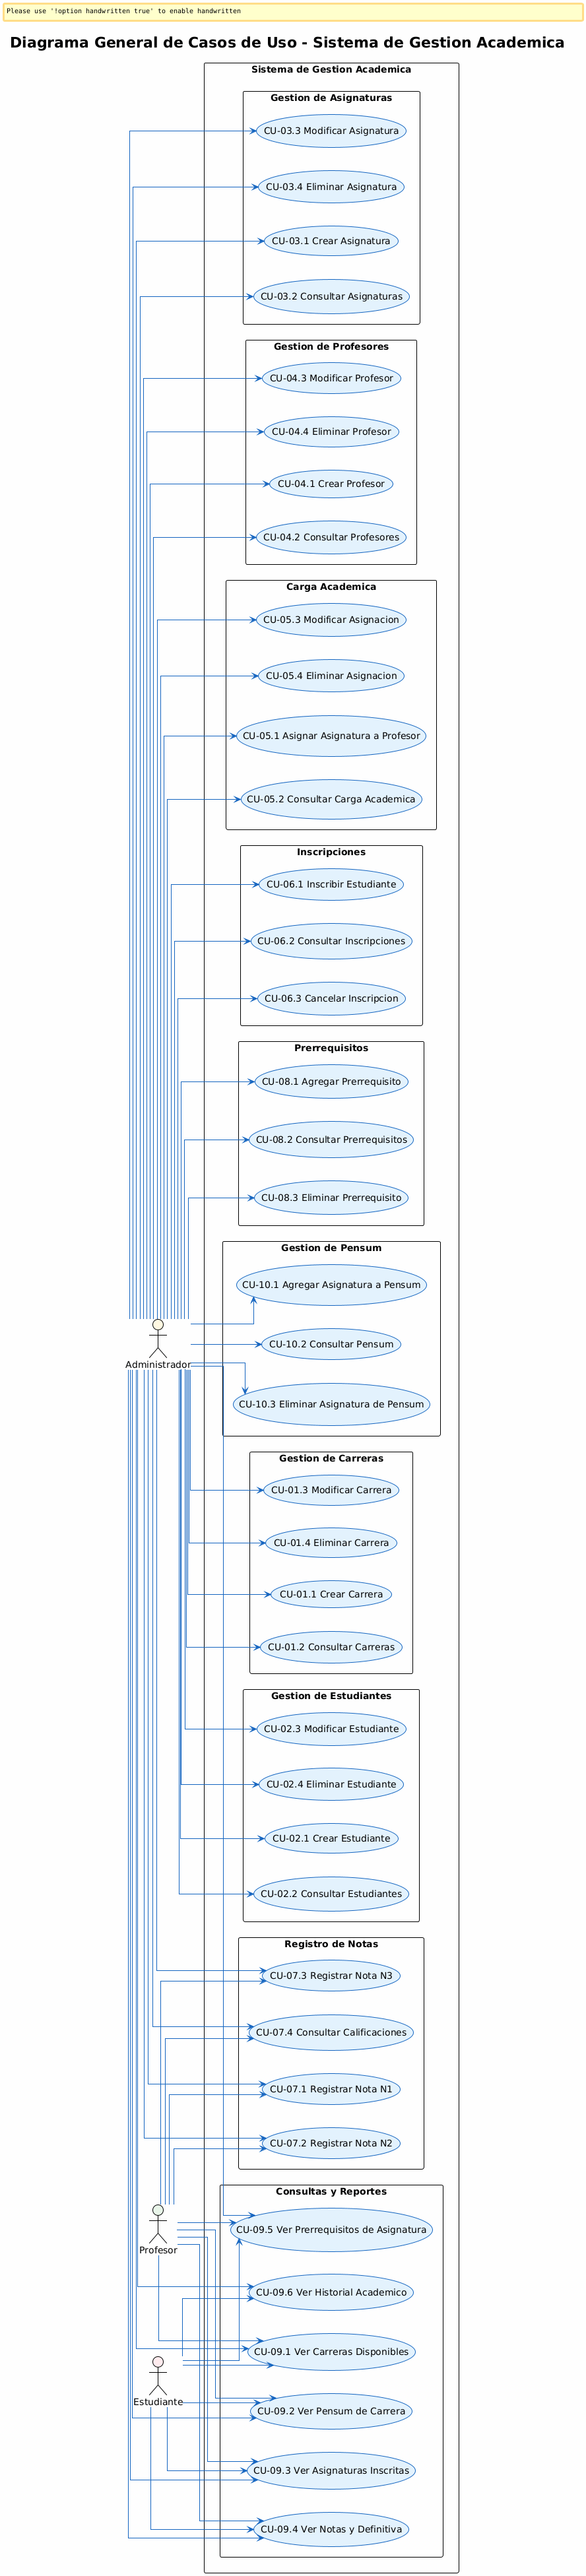
\includegraphics[width=\textwidth]{01_diagrama_general_casos_uso.png}
    \caption{Diagrama General de Casos de Uso - Sistema de Gestion Academica}
    \label{fig:general}
\end{figure}

\subsection{Casos de Uso por Actor}

\subsubsection{Casos de Uso del Administrador}

El administrador tiene acceso total a todas las funcionalidades del sistema. La figura \ref{fig:admin} detalla los casos de uso especificos del administrador.

\begin{figure}[H]
    \centering
    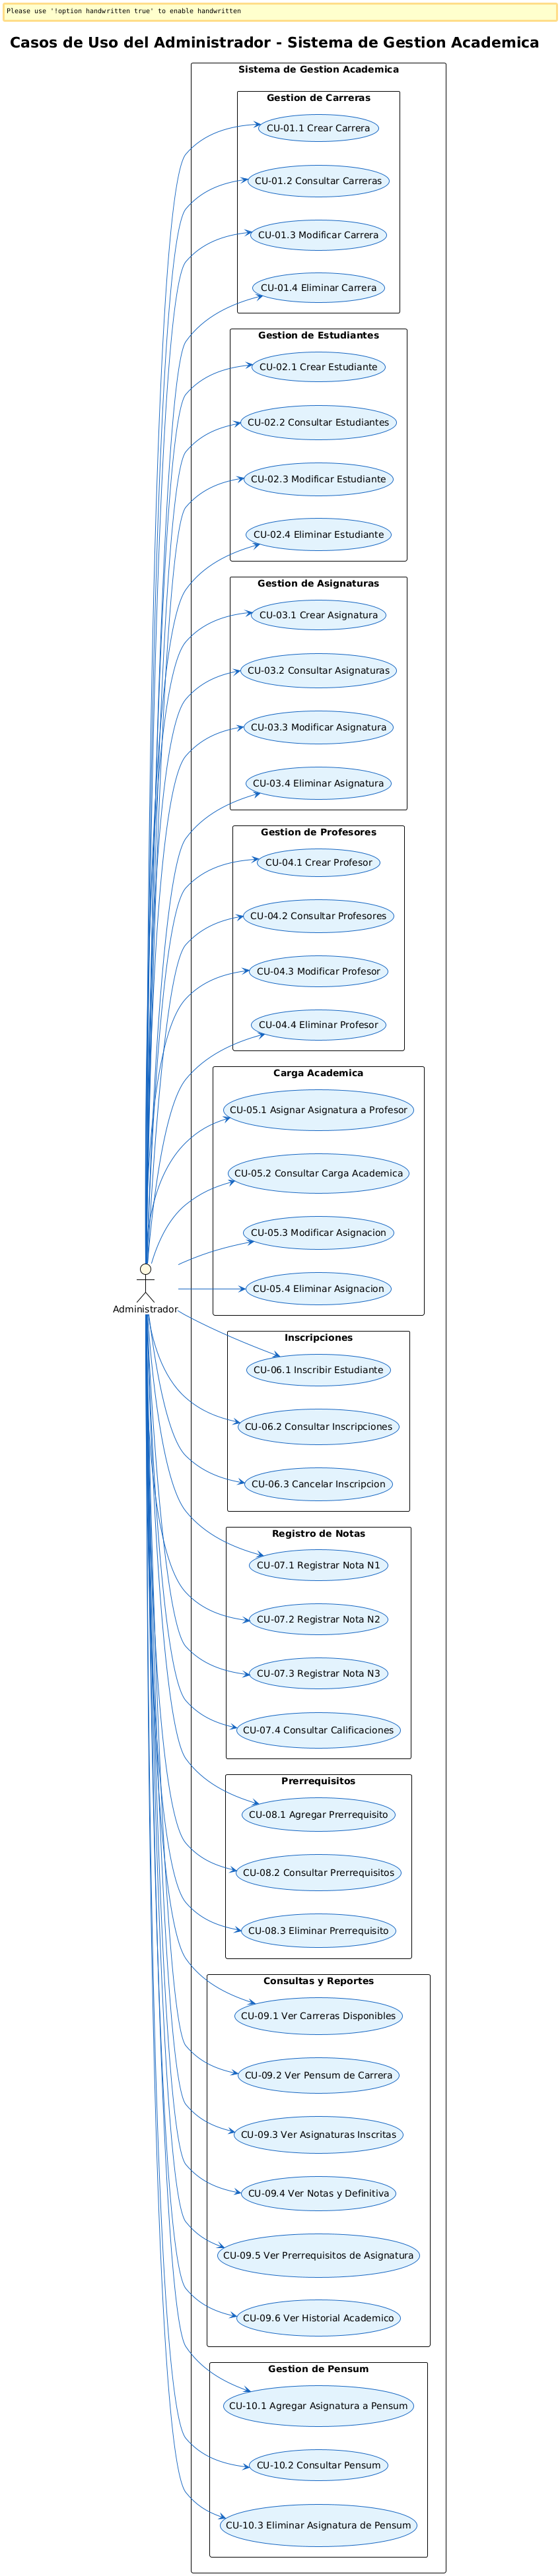
\includegraphics[width=\textwidth]{02_casos_uso_administrador.png}
    \caption{Casos de Uso del Administrador}
    \label{fig:admin}
\end{figure}

\subsubsection{Casos de Uso del Profesor}

El profesor tiene acceso limitado para registrar notas y consultar informacion academica. La figura \ref{fig:profesor} muestra sus casos de uso.

\begin{figure}[H]
    \centering
    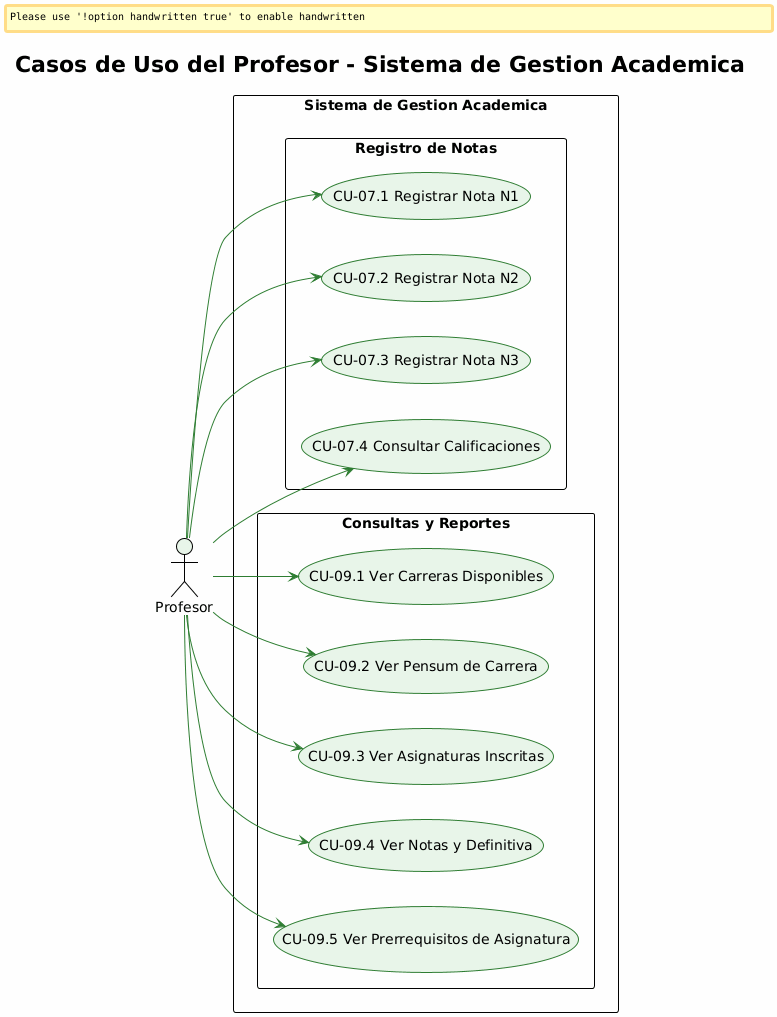
\includegraphics[width=0.85\textwidth]{03_casos_uso_profesor.png}
    \caption{Casos de Uso del Profesor}
    \label{fig:profesor}
\end{figure}

\subsubsection{Casos de Uso del Estudiante}

El estudiante solo puede consultar informacion relacionada con su situacion academica. La figura \ref{fig:estudiante} presenta sus casos de uso.

\begin{figure}[H]
    \centering
    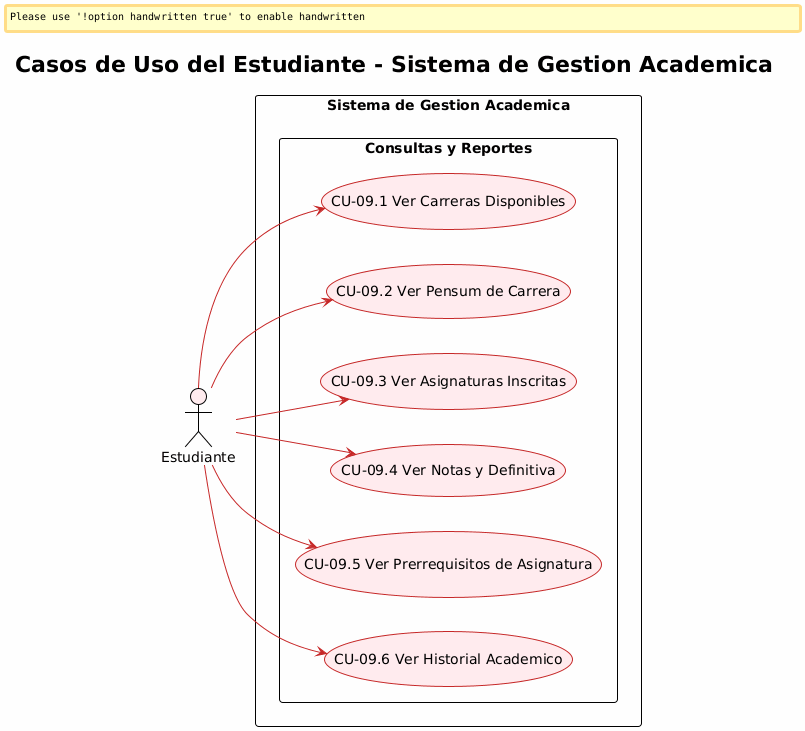
\includegraphics[width=0.85\textwidth]{04_casos_uso_estudiante.png}
    \caption{Casos de Uso del Estudiante}
    \label{fig:estudiante}
\end{figure}

\subsection{Detalle de Subsistemas}

A continuacion se presentan los diagramas de casos de uso detallados por subsistema, incluyendo relaciones de inclusion (\textless\textless include\textgreater\textgreater) y extension (\textless\textless extend\textgreater\textgreater).

\subsubsection{Subsistema de Gestion de Carreras}

\begin{figure}[H]
    \centering
    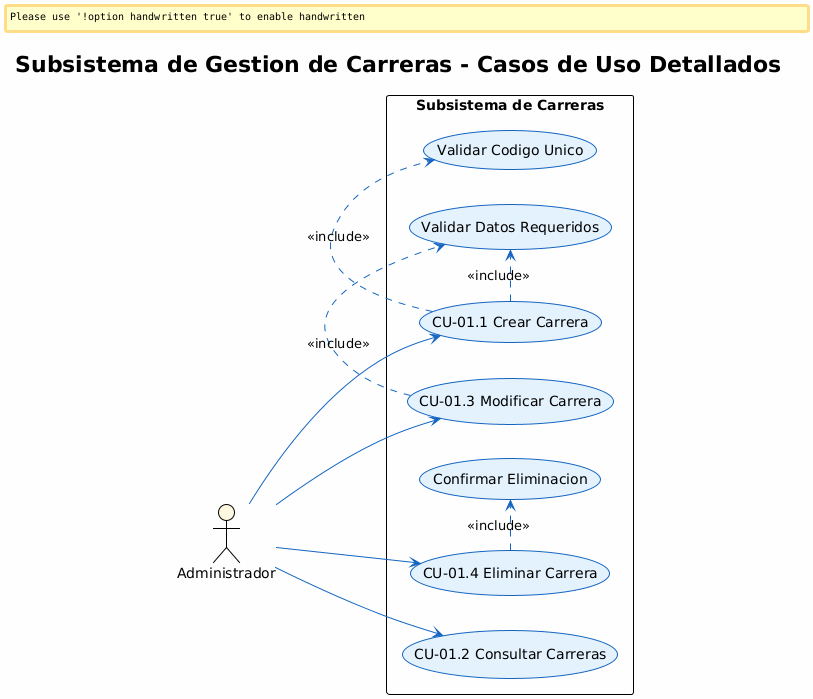
\includegraphics[width=0.8\textwidth]{05_subsistema_carreras.png}
    \caption{Subsistema de Gestion de Carreras}
    \label{fig:carreras}
\end{figure}

\textbf{Descripcion de casos de uso:}
\begin{itemize}
    \item \textbf{CU-01.1 Crear Carrera}: Permite al administrador registrar una nueva carrera academica en el sistema. Incluye la validacion de codigo unico y datos requeridos.
    \item \textbf{CU-01.2 Consultar Carreras}: Permite visualizar el listado de carreras registradas con sus atributos.
    \item \textbf{CU-01.3 Modificar Carrera}: Permite actualizar la informacion de una carrera existente.
    \item \textbf{CU-01.4 Eliminar Carrera}: Permite eliminar una carrera previa confirmacion.
\end{itemize}

\subsubsection{Subsistema de Gestion de Estudiantes}

\begin{figure}[H]
    \centering
    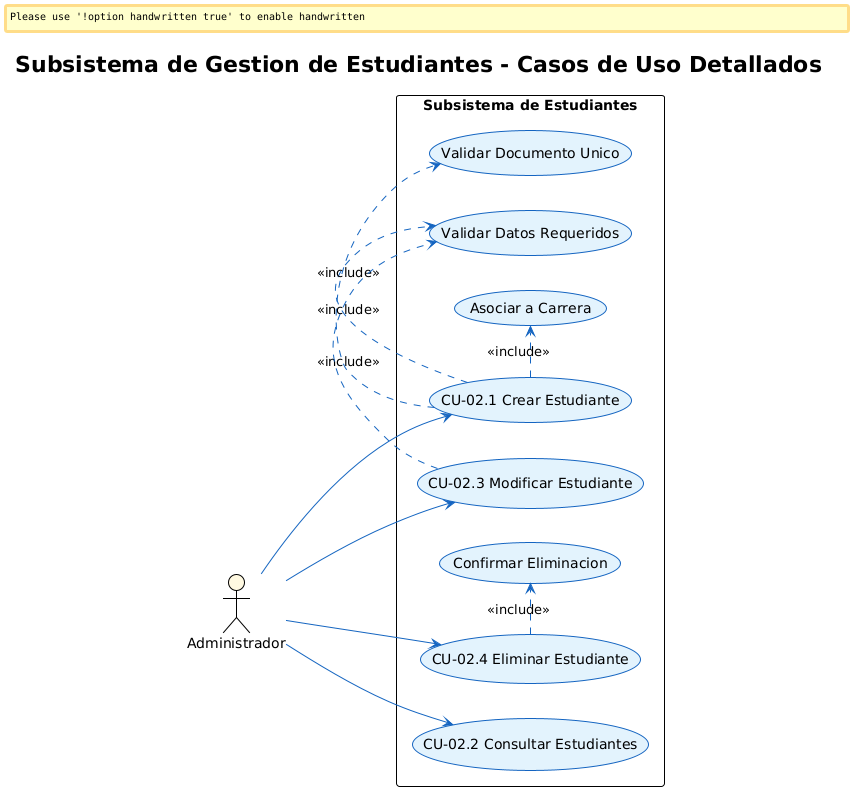
\includegraphics[width=0.8\textwidth]{06_subsistema_estudiantes.png}
    \caption{Subsistema de Gestion de Estudiantes}
    \label{fig:estudiantes}
\end{figure}

\textbf{Descripcion de casos de uso:}
\begin{itemize}
    \item \textbf{CU-02.1 Crear Estudiante}: Registra un nuevo estudiante validando documento unico y asociandolo a una carrera.
    \item \textbf{CU-02.2 Consultar Estudiantes}: Visualiza el listado de estudiantes con filtros por carrera.
    \item \textbf{CU-02.3 Modificar Estudiante}: Actualiza datos personales y academicos del estudiante.
    \item \textbf{CU-02.4 Eliminar Estudiante}: Elimina un estudiante previa confirmacion.
\end{itemize}

\subsubsection{Subsistema de Gestion de Asignaturas}

\begin{figure}[H]
    \centering
    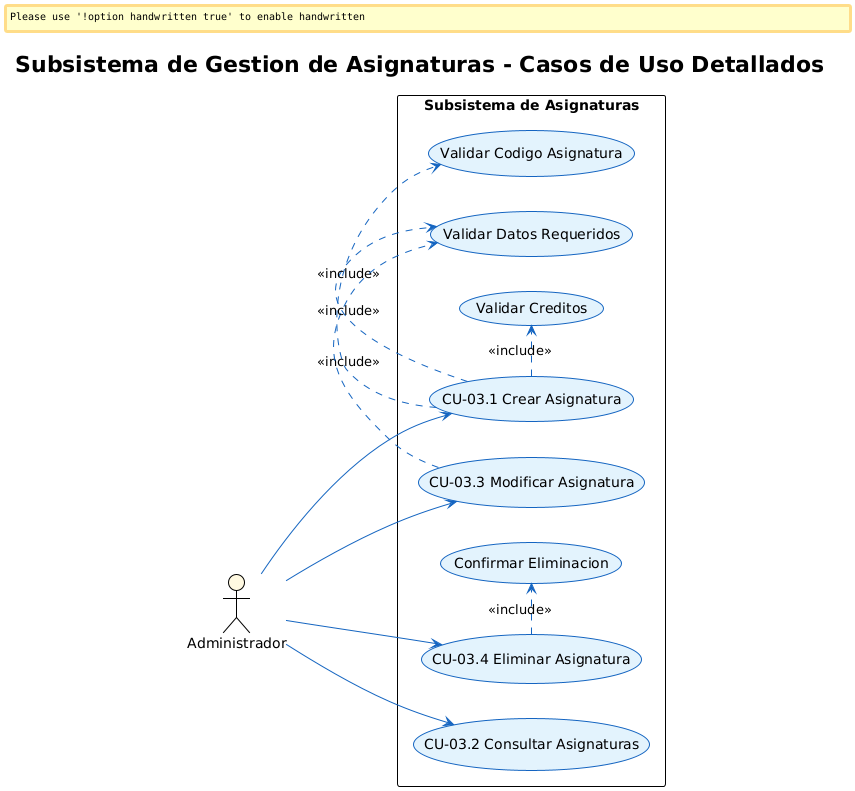
\includegraphics[width=0.8\textwidth]{07_subsistema_asignaturas.png}
    \caption{Subsistema de Gestion de Asignaturas}
    \label{fig:asignaturas}
\end{figure}

\textbf{Descripcion de casos de uso:}
\begin{itemize}
    \item \textbf{CU-03.1 Crear Asignatura}: Registra una nueva asignatura con codigo, nombre y creditos.
    \item \textbf{CU-03.2 Consultar Asignaturas}: Lista todas las asignaturas del catalogo.
    \item \textbf{CU-03.3 Modificar Asignatura}: Actualiza atributos de una asignatura.
    \item \textbf{CU-03.4 Eliminar Asignatura}: Elimina una asignatura del catalogo.
\end{itemize}

\subsubsection{Subsistema de Gestion de Profesores}

\begin{figure}[H]
    \centering
    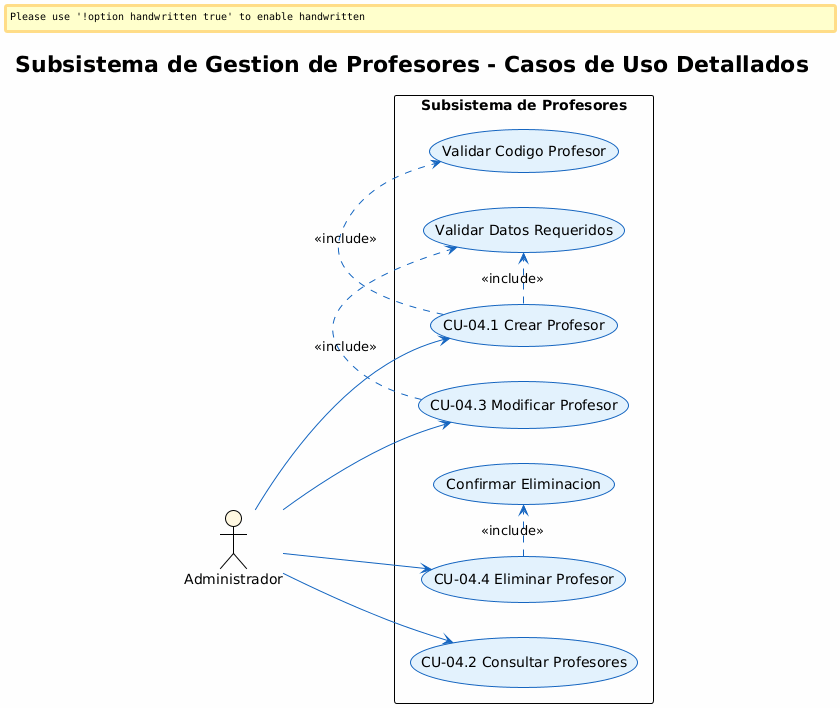
\includegraphics[width=0.8\textwidth]{08_subsistema_profesores.png}
    \caption{Subsistema de Gestion de Profesores}
    \label{fig:profesores}
\end{figure}

\textbf{Descripcion de casos de uso:}
\begin{itemize}
    \item \textbf{CU-04.1 Crear Profesor}: Registra un nuevo profesor en el sistema.
    \item \textbf{CU-04.2 Consultar Profesores}: Visualiza el listado de profesores activos.
    \item \textbf{CU-04.3 Modificar Profesor}: Actualiza informacion del profesor.
    \item \textbf{CU-04.4 Eliminar Profesor}: Elimina un profesor del sistema.
\end{itemize}

\subsubsection{Subsistema de Carga Academica}

\begin{figure}[H]
    \centering
    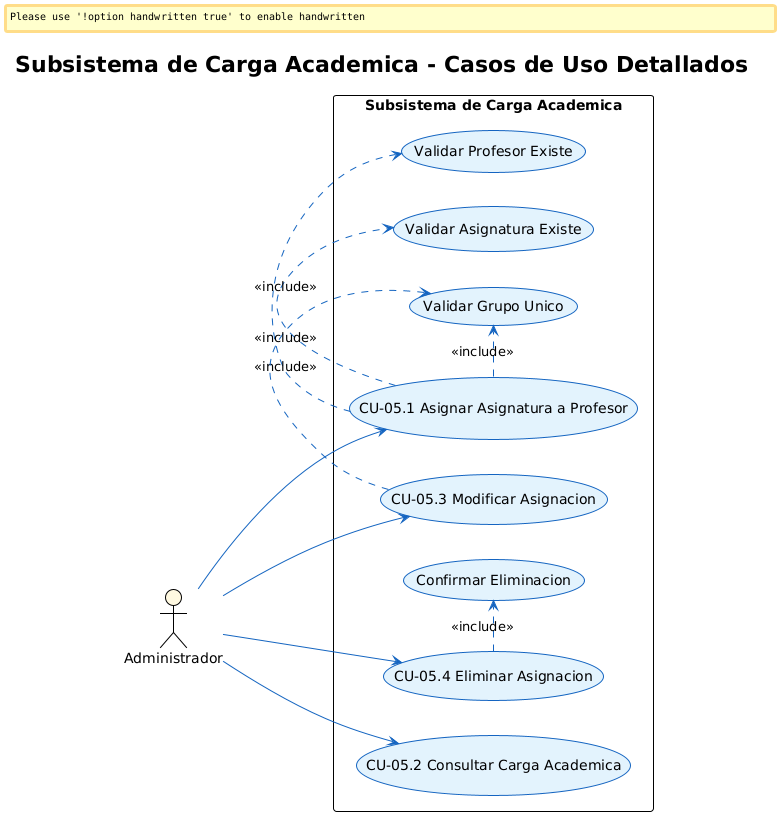
\includegraphics[width=0.8\textwidth]{09_subsistema_carga_academica.png}
    \caption{Subsistema de Carga Academica}
    \label{fig:carga}
\end{figure}

\textbf{Descripcion de casos de uso:}
\begin{itemize}
    \item \textbf{CU-05.1 Asignar Asignatura a Profesor}: Asocia una asignatura a un profesor para un grupo especifico.
    \item \textbf{CU-05.2 Consultar Carga Academica}: Visualiza las asignaciones actuales.
    \item \textbf{CU-05.3 Modificar Asignacion}: Cambia profesor o grupo de una asignacion.
    \item \textbf{CU-05.4 Eliminar Asignacion}: Elimina una asignacion de carga academica.
\end{itemize}

\subsubsection{Subsistema de Inscripciones}

\begin{figure}[H]
    \centering
    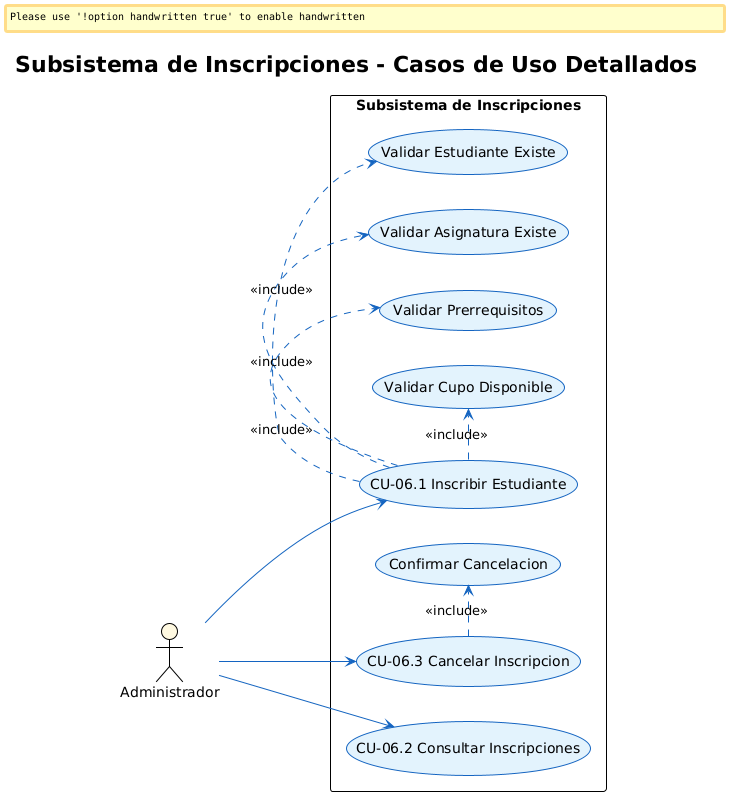
\includegraphics[width=0.8\textwidth]{10_subsistema_inscripciones.png}
    \caption{Subsistema de Inscripciones}
    \label{fig:inscripciones}
\end{figure}

\textbf{Descripcion de casos de uso:}
\begin{itemize}
    \item \textbf{CU-06.1 Inscribir Estudiante}: Inscribe un estudiante a una asignatura validando prerrequisitos y cupo. Utiliza el stored procedure \texttt{sp\_inscribir\_estudiante}.
    \item \textbf{CU-06.2 Consultar Inscripciones}: Lista las inscripciones activas por periodo.
    \item \textbf{CU-06.3 Cancelar Inscripcion}: Cancela una inscripcion previa confirmacion.
\end{itemize}

\subsubsection{Subsistema de Registro de Notas}

\begin{figure}[H]
    \centering
    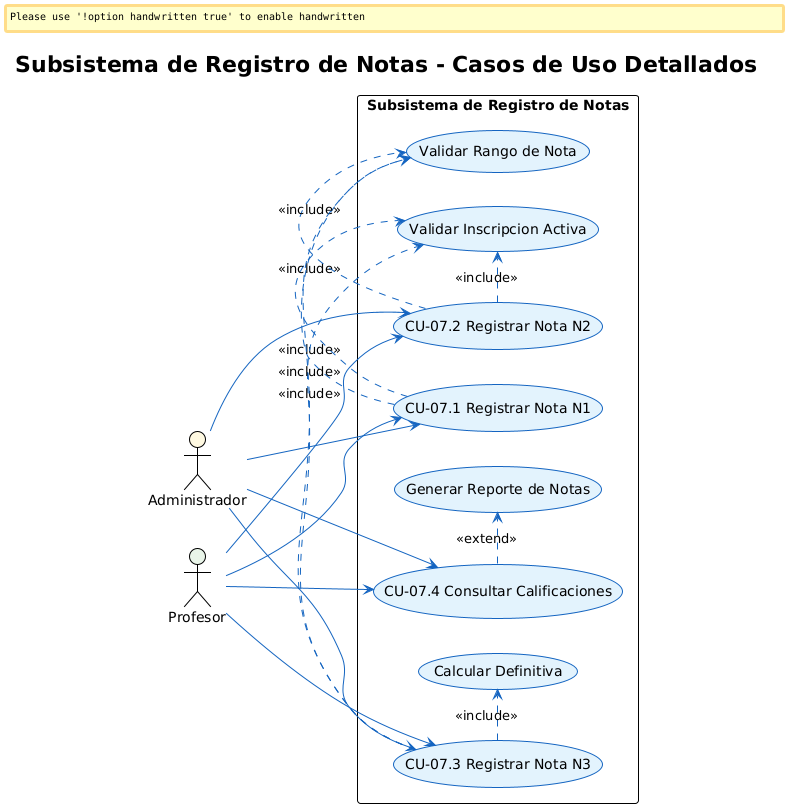
\includegraphics[width=0.85\textwidth]{11_subsistema_notas.png}
    \caption{Subsistema de Registro de Notas}
    \label{fig:notas}
\end{figure}

\textbf{Descripcion de casos de uso:}
\begin{itemize}
    \item \textbf{CU-07.1 Registrar Nota N1}: Registra la nota del primer corte (35\%).
    \item \textbf{CU-07.2 Registrar Nota N2}: Registra la nota del segundo corte (35\%).
    \item \textbf{CU-07.3 Registrar Nota N3}: Registra la nota del tercer corte (30\%). El trigger \texttt{trg\_calculo\_notas} calcula automaticamente la definitiva.
    \item \textbf{CU-07.4 Consultar Calificaciones}: Visualiza las notas registradas y la definitiva calculada.
\end{itemize}

La formula de calculo de la nota definitiva es:
\begin{equation}
    Definitiva = (n_1 \times 0.35) + (n_2 \times 0.35) + (n_3 \times 0.30)
\end{equation}

\subsubsection{Subsistema de Prerrequisitos}

\begin{figure}[H]
    \centering
    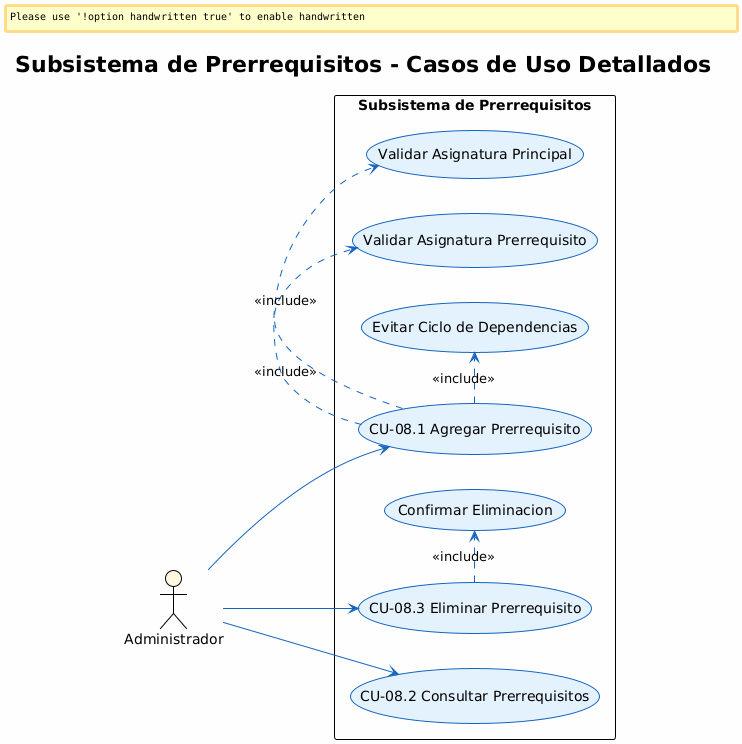
\includegraphics[width=0.8\textwidth]{12_subsistema_prerrequisitos.png}
    \caption{Subsistema de Prerrequisitos}
    \label{fig:prerrequisitos}
\end{figure}

\textbf{Descripcion de casos de uso:}
\begin{itemize}
    \item \textbf{CU-08.1 Agregar Prerrequisito}: Define una asignatura como prerrequisito de otra, validando que no se creen ciclos de dependencia.
    \item \textbf{CU-08.2 Consultar Prerrequisitos}: Visualiza la cadena de prerrequisitos de una asignatura.
    \item \textbf{CU-08.3 Eliminar Prerrequisito}: Elimina una relacion de prerrequisito.
\end{itemize}

\subsubsection{Subsistema de Gestion de Pensum}

\begin{figure}[H]
    \centering
    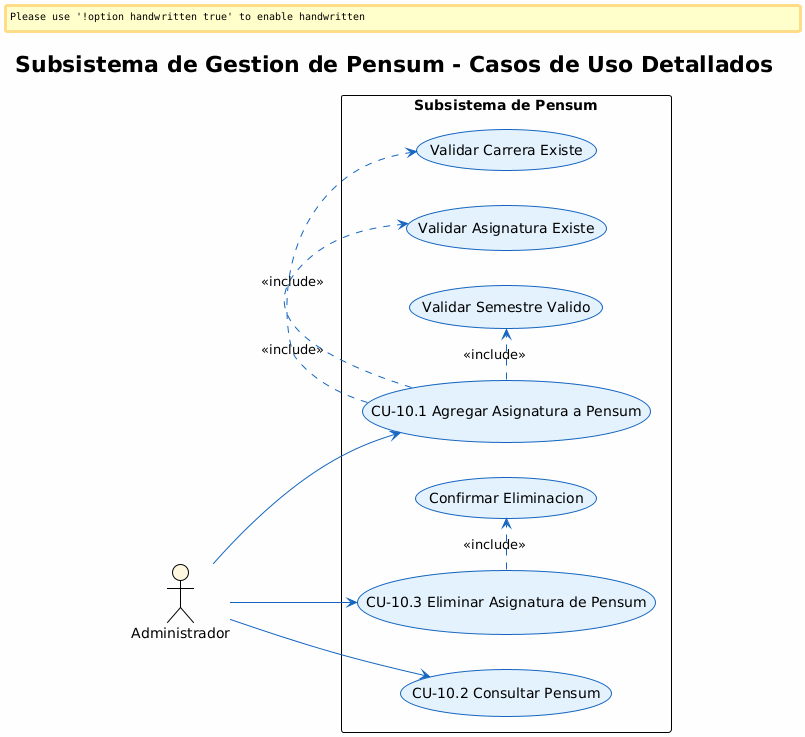
\includegraphics[width=0.8\textwidth]{13_subsistema_pensum.png}
    \caption{Subsistema de Gestion de Pensum}
    \label{fig:pensum}
\end{figure}

\textbf{Descripcion de casos de uso:}
\begin{itemize}
    \item \textbf{CU-10.1 Agregar Asignatura a Pensum}: Asocia una asignatura a una carrera en un semestre especifico.
    \item \textbf{CU-10.2 Consultar Pensum}: Visualiza el pensum completo de una carrera organizado por semestres.
    \item \textbf{CU-10.3 Eliminar Asignatura de Pensum}: Elimina una asignatura del pensum de una carrera.
\end{itemize}

\subsubsection{Subsistema de Consultas y Reportes}

\begin{figure}[H]
    \centering
    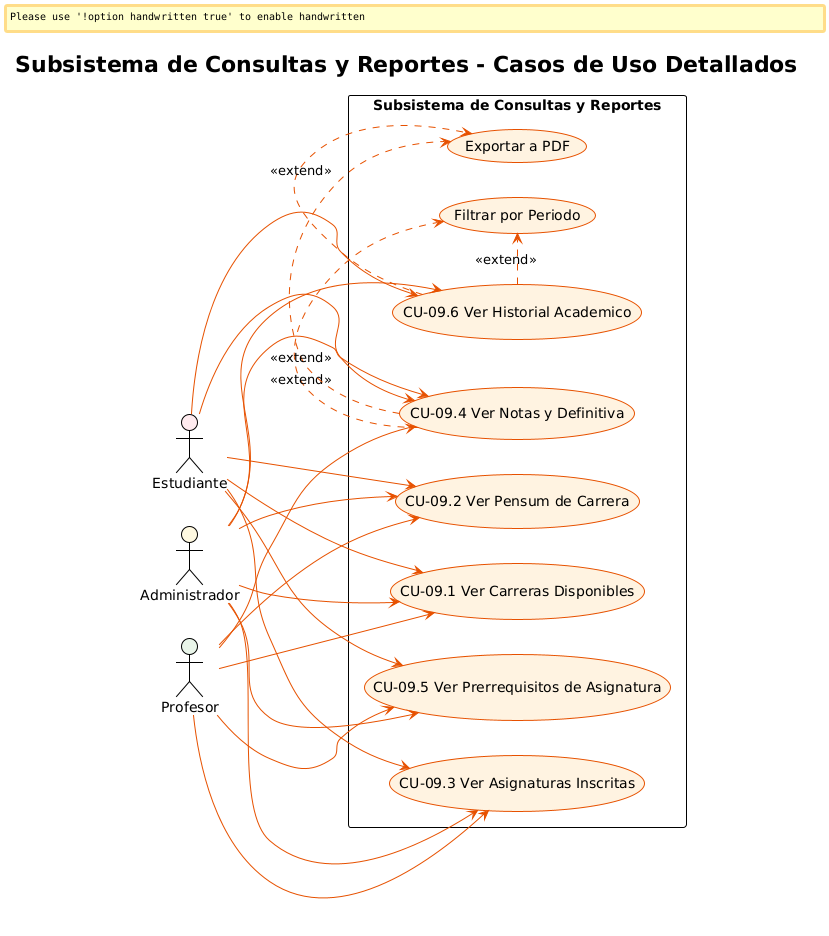
\includegraphics[width=0.85\textwidth]{14_subsistema_consultas.png}
    \caption{Subsistema de Consultas y Reportes}
    \label{fig:consultas}
\end{figure}

\textbf{Descripcion de casos de uso:}
\begin{itemize}
    \item \textbf{CU-09.1 Ver Carreras Disponibles}: Lista las carreras activas del sistema.
    \item \textbf{CU-09.2 Ver Pensum de Carrera}: Muestra el pensum detallado de una carrera especifica.
    \item \textbf{CU-09.3 Ver Asignaturas Inscritas}: Lista las asignaturas en las que el estudiante esta inscrito.
    \item \textbf{CU-09.4 Ver Notas y Definitiva}: Muestra las calificaciones del estudiante con la nota definitiva.
    \item \textbf{CU-09.5 Ver Prerrequisitos de Asignatura}: Consulta los prerrequisitos de una asignatura especifica.
    \item \textbf{CU-09.6 Ver Historial Academico}: Muestra el historial completo de notas y asignaturas cursadas.
\end{itemize}

\subsection{Matriz de Trazabilidad de Casos de Uso}

La figura \ref{fig:matriz} presenta la matriz de trazabilidad que relaciona cada caso de uso con los actores que tienen permiso para ejecutarlo.

\begin{figure}[H]
    \centering
    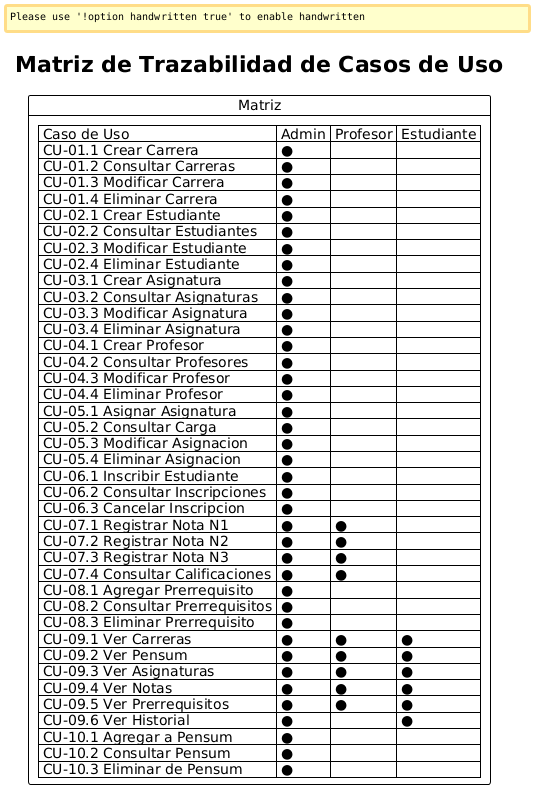
\includegraphics[width=\textwidth]{15_matriz_trazabilidad.png}
    \caption{Matriz de Trazabilidad de Casos de Uso}
    \label{fig:matriz}
\end{figure}

\textbf{Resumen de acceso por rol:}
\begin{itemize}
    \item \textbf{Administrador}: Acceso total a los 37 casos de uso del sistema.
    \item \textbf{Profesor}: Acceso a 9 casos de uso (registro de notas y consultas).
    \item \textbf{Estudiante}: Acceso a 6 casos de uso (consultas de solo lectura).
\end{itemize}


%===============================================================================
% VISTA LOGICA
%===============================================================================
\newpage
\section{Vista Logica}

\subsection{Descripcion General}

La vista logica describe la estructura estatica del sistema mediante clases, paquetes y sus relaciones. El sistema sigue una arquitectura en capas con separacion clara entre presentacion, control, modelo y acceso a datos.

\subsection{Estructura de Paquetes}

El codigo fuente Java esta organizado en los siguientes paquetes:

\begin{lstlisting}[language=Java, caption=Estructura de paquetes del sistema]
com.academico/
|-- config/          # Configuracion de conexion a BD (Singleton)
|-- controller/      # Controladores JavaFX (MVC)
|-- dao/             # Data Access Objects
|-- model/           # Entidades del dominio
|-- Main.java        # Punto de entrada
\end{lstlisting}

\subsection{Descripcion de Clases Principales}

\subsubsection{Capa de Modelo (Model)}

Las clases del modelo representan las entidades del dominio academico:

\begin{longtable}{|p{4cm}|p{10cm}|}
\hline
\rowcolor{udgreen!20}
\textbf{Clase} & \textbf{Descripcion y Atributos Principales} \\
\hline
\endfirsthead
\hline
\rowcolor{udgreen!20}
\textbf{Clase} & \textbf{Descripcion y Atributos Principales} \\
\hline
\endhead
Carrera & Representa una carrera academica. Atributos: codigo, nombre, numero de semestres. \\
\hline
Estudiante & Representa un estudiante. Atributos: codigo, nombre, carrera (FK). \\
\hline
Asignatura & Representa una asignatura del catalogo. Atributos: codigo, nombre, creditos. \\
\hline
Profesor & Representa un profesor. Atributos: codigo, nombre, especialidad. \\
\hline
Imparte & Representa la asignacion de una asignatura a un profesor. Atributos: profesor, asignatura, grupo, anio, periodo. \\
\hline
Inscripcion & Representa la inscripcion de un estudiante. Atributos: estudiante, asignatura, notas (n1, n2, n3, definitiva). \\
\hline
Pensum & Relacion entre carrera y asignatura. Atributos: carrera, asignatura, semestre. \\
\hline
Prerrequisito & Relacion de dependencia entre asignaturas. Atributos: asignatura, prerrequisito. \\
\hline
\end{longtable}

\subsubsection{Capa de Acceso a Datos (DAO)}

Cada entidad del modelo cuenta con un DAO correspondiente que implementa las operaciones CRUD:

\begin{itemize}
    \item \textbf{CarreraDAO}: Operaciones CRUD para carreras.
    \item \textbf{EstudianteDAO}: Operaciones CRUD para estudiantes.
    \item \textbf{AsignaturaDAO}: Operaciones CRUD para asignaturas.
    \item \textbf{ProfesorDAO}: Operaciones CRUD para profesores.
    \item \textbf{ImparteDAO}: Operaciones para asignar y gestionar carga academica.
    \item \textbf{InscripcionDAO}: Operaciones de inscripcion y registro de notas.
    \item \textbf{PensumDAO}: Operaciones de gestion de pensum.
    \item \textbf{PrerrequisitoDAO}: Operaciones de gestion de prerrequisitos.
\end{itemize}

\subsubsection{Clase OperationResult}

La clase \texttt{OperationResult} encapsula el resultado de cualquier operacion de base de datos:

\begin{lstlisting}[language=Java, caption=Clase OperationResult]
public class OperationResult<T> {
    private boolean success;
    private String message;
    private T data;
    
    public static <T> OperationResult<T> success(T data, String message) { ... }
    public static <T> OperationResult<T> error(String message) { ... }
}
\end{lstlisting}

Esta clase permite propagar mensajes de exito o error desde la base de datos hasta la interfaz de usuario de forma uniforme.

\subsection{Patrones de Diseno Aplicados}

\subsubsection{Patron Singleton}

La clase \texttt{DatabaseConfig} implementa el patron Singleton para garantizar una unica conexion a la base de datos:

\begin{lstlisting}[language=Java, caption=Implementacion del patron Singleton]
public class DatabaseConfig {
    private static DatabaseConfig instance;
    private Connection connection;
    
    private DatabaseConfig() { ... }
    
    public static synchronized DatabaseConfig getInstance() {
        if (instance == null) {
            instance = new DatabaseConfig();
        }
        return instance;
    }
}
\end{lstlisting}

\subsubsection{Patron DAO}

Cada DAO sigue una estructura consistente. Ejemplo de CarreraDAO:

\begin{lstlisting}[language=Java, caption=Patron DAO - CarreraDAO]
public class CarreraDAO {
    private Connection connection;
    
    public OperationResult<Carrera> crear(Carrera carrera) { ... }
    public OperationResult<List<Carrera>> consultarTodas() { ... }
    public OperationResult<Carrera> consultarPorCodigo(String codigo) { ... }
    public OperationResult<Void> modificar(Carrera carrera) { ... }
    public OperationResult<Void> eliminar(String codigo) { ... }
}
\end{lstlisting}

%===============================================================================
% VISTA DE PROCESOS
%===============================================================================
\newpage
\section{Vista de Procesos}

\subsection{Descripcion General}

La vista de procesos describe la dinamica del sistema, mostrando como los componentes interactuan en tiempo de ejecucion para cumplir con las funcionalidades definidas en los casos de uso.

\subsection{Flujo de Inscripcion de Estudiante}

El flujo de inscripcion es uno de los mas criticos del sistema, ya que involucra validaciones de prerrequisitos mediante el stored procedure \texttt{sp\_inscribir\_estudiante}:

\begin{enumerate}
    \item El administrador selecciona el estudiante y la asignatura a inscribir.
    \item El sistema invoca \texttt{sp\_inscribir\_estudiante(estudiante, asignatura)}.
    \item El stored procedure verifica que el estudiante exista.
    \item El SP verifica que la asignatura exista.
    \item El SP valida que el estudiante haya aprobado todos los prerrequisitos.
    \item Si la validacion falla, lanza \texttt{RAISE EXCEPTION} con mensaje descriptivo.
    \item Si la validacion es exitosa, inserta el registro en la tabla Inscribe.
    \item El trigger \texttt{trg\_calculo\_notas} inicializa las notas en NULL.
    \item El sistema recibe el mensaje de exito y lo muestra al usuario.
\end{enumerate}

\subsection{Flujo de Registro de Notas}

El registro de notas dispara automaticamente el calculo de la nota definitiva:

\begin{enumerate}
    \item El profesor o administrador ingresa la nota N1, N2 o N3.
    \item El sistema ejecuta \texttt{UPDATE Inscribe SET nX = valor}.
    \item El trigger \texttt{trg\_calculo\_notas} se activa despues del UPDATE.
    \item El trigger calcula: \texttt{definitiva = (n1 * 0.35) + (n2 * 0.35) + (n3 * 0.30)}.
    \item El trigger actualiza el campo definitiva automaticamente.
    \item El sistema confirma la operacion al usuario.
\end{enumerate}

\subsection{Flujo de Autenticacion}

\begin{enumerate}
    \item El usuario selecciona su rol (Administrador, Profesor o Estudiante).
    \item El sistema establece la conexion a PostgreSQL con las credenciales correspondientes:
    \begin{itemize}
        \item \texttt{app\_admin / Admin\_Secret2026*}
        \item \texttt{app\_profesor / Prof\_Secret2026*}
        \item \texttt{app\_estudiante / Est\_Secret2026*}
    \end{itemize}
    \item PostgreSQL verifica el rol y aplica los permisos RBAC correspondientes.
    \item El sistema carga la interfaz acorde al rol autenticado.
\end{enumerate}

%===============================================================================
% VISTA DE DESPLIEGUE
%===============================================================================
\newpage
\section{Vista de Despliegue}

\subsection{Descripcion de la Infraestructura}

El sistema se despliega en una arquitectura de dos capas:

\begin{enumerate}
    \item \textbf{Capa de Cliente}: Aplicacion de escritorio JavaFX ejecutandose en la maquina del usuario.
    \item \textbf{Capa de Datos}: Base de datos PostgreSQL 15 ejecutandose en un contenedor Docker.
\end{enumerate}

\subsection{Configuracion de Hardware y Software}

\begin{longtable}{|p{3cm}|p{5cm}|p{6cm}|}
\hline
\rowcolor{udgreen!20}
\textbf{Nodo} & \textbf{Hardware Minimo} & \textbf{Software Requerido} \\
\hline
\endfirsthead
\hline
\rowcolor{udgreen!20}
\textbf{Nodo} & \textbf{Hardware Minimo} & \textbf{Software Requerido} \\
\hline
\endhead
Cliente & CPU: 2 cores, RAM: 4 GB, Disco: 1 GB & Java 17, JavaFX, Maven 3.8 \\
\hline
Servidor BD & CPU: 2 cores, RAM: 2 GB, Disco: 10 GB & Docker, Docker Compose, PostgreSQL 15 \\
\hline
\end{longtable}

\subsection{Diagrama de Despliegue}

La configuracion de despliegue se describe textualmente dado que es una arquitectura simple de dos nodos:

\begin{itemize}
    \item \textbf{Nodo Cliente}: Ejecuta la aplicacion JavaFX. Se comunica con el servidor de base de datos mediante JDBC a traves del puerto 5432.
    \item \textbf{Nodo Servidor PostgreSQL}: Contenedor Docker que expone el puerto 5432. Incluye scripts de inicializacion en \texttt{init-scripts/} que crean el esquema, tablas, triggers, stored procedures, roles y datos de prueba.
\end{itemize}

\subsection{Configuracion de Red}

\begin{itemize}
    \item \textbf{Protocolo}: TCP/IP
    \item \textbf{Puerto de BD}: 5432
    \item \textbf{Driver JDBC}: PostgreSQL JDBC 42.7.3
    \item \textbf{Host}: localhost (o IP del contenedor Docker)
\end{itemize}

%===============================================================================
% VISTA DE DATOS
%===============================================================================
\newpage
\section{Vista de Datos}

\subsection{Modelo Entidad-Relacion}

La base de datos del sistema sigue el siguiente modelo relacional:

\begin{longtable}{|p{3cm}|p{11cm}|}
\hline
\rowcolor{udgreen!20}
\textbf{Tabla} & \textbf{Descripcion y Atributos} \\
\hline
\endfirsthead
\hline
\rowcolor{udgreen!20}
\textbf{Tabla} & \textbf{Descripcion y Atributos} \\
\hline
\endhead
Carreras & codigo (PK), nombre, num\_semestres \\
\hline
Estudiantes & codigo (PK), nombre, cod\_carrera (FK) \\
\hline
Asignaturas & codigo (PK), nombre, creditos \\
\hline
Profesores & codigo (PK), nombre, especialidad \\
\hline
Imparte & codigo (PK), cod\_profesor (FK), cod\_asignatura (FK), grupo, anio, periodo \\
\hline
Inscribe & codigo (PK), cod\_estudiante (FK), cod\_asignatura (FK), n1, n2, n3, definitiva \\
\hline
Incluye & codigo (PK), cod\_carrera (FK), cod\_asignatura (FK), semestre \\
\hline
Requiere & codigo (PK), cod\_asignatura (FK), cod\_prerrequisito (FK) \\
\hline
\end{longtable}

\subsection{Restricciones de Integridad}

\begin{itemize}
    \item \textbf{Claves primarias}: Todas las tablas tienen un campo codigo como clave primaria.
    \item \textbf{Claves foraneas}: Las relaciones entre tablas garantizan la integridad referencial.
    \item \textbf{Regla de negocio}: La nota definitiva se calcula automaticamente mediante trigger.
    \item \textbf{Validacion}: Los prerrequisitos se validan mediante stored procedure antes de la inscripcion.
\end{itemize}

\subsection{Triggers y Stored Procedures}

\subsubsection{Trigger trg\_calculo\_notas}

\begin{lstlisting}[language=SQL, caption=Trigger de calculo de notas definitivas]
CREATE TRIGGER trg_calculo_notas
AFTER INSERT OR UPDATE OF n1, n2, n3 ON Inscribe
FOR EACH ROW
EXECUTE FUNCTION calcular_definitiva();
\end{lstlisting}

\subsubsection{Stored Procedure sp\_inscribir\_estudiante}

\begin{lstlisting}[language=SQL, caption=Stored Procedure de validacion de inscripcion]
CREATE OR REPLACE PROCEDURE sp_inscribir_estudiante(
    p_estudiante VARCHAR,
    p_asignatura VARCHAR
)
LANGUAGE plpgsql
AS $$
BEGIN
    -- Validar prerrequisitos
    IF EXISTS (
        SELECT 1 FROM Requiere r
        WHERE r.cod_asignatura = p_asignatura
        AND r.cod_prerrequisito NOT IN (
            SELECT i.cod_asignatura FROM Inscribe i
            WHERE i.cod_estudiante = p_estudiante
            AND i.definitiva >= 3.0
        )
    ) THEN
        RAISE EXCEPTION 'El estudiante no ha aprobado todos los prerrequisitos';
    END IF;
    
    -- Realizar inscripcion
    INSERT INTO Inscribe (cod_estudiante, cod_asignatura, n1, n2, n3)
    VALUES (p_estudiante, p_asignatura, NULL, NULL, NULL);
END;
$$;
\end{lstlisting}

\subsection{Control de Acceso (RBAC)}

El sistema implementa tres roles de PostgreSQL con permisos diferenciados:

\begin{longtable}{|p{4cm}|p{10cm}|}
\hline
\rowcolor{udgreen!20}
\textbf{Rol} & \textbf{Privilegios} \\
\hline
\endfirsthead
\hline
\rowcolor{udgreen!20}
\textbf{Rol} & \textbf{Privilegios} \\
\hline
\endhead
rol\_admin\_academico & Control total (SELECT, INSERT, UPDATE, DELETE) sobre todas las tablas. \\
\hline
rol\_profesor & SELECT en todas las tablas, UPDATE solo en Inscribe (notas). \\
\hline
rol\_estudiante & SELECT en Carreras, Asignaturas, Incluye, Requiere (solo lectura). \\
\hline
\end{longtable}

%===============================================================================
% TAMANO Y RENDIMIENTO
%===============================================================================
\newpage
\section{Tamano y Rendimiento}

\subsection{Estimacion de Tamano}

\begin{longtable}{|p{5cm}|p{3cm}|p{6cm}|}
\hline
\rowcolor{udgreen!20}
\textbf{Componente} & \textbf{Estimacion} & \textbf{Observaciones} \\
\hline
\endfirsthead
\hline
\rowcolor{udgreen!20}
\textbf{Componente} & \textbf{Estimacion} & \textbf{Observaciones} \\
\hline
\endhead
Lineas de codigo Java & Aprox. 5,000 & Incluye modelo, DAO, controladores y utilidades \\
\hline
Lineas de codigo SQL & Aprox. 1,500 & DDL, DML, triggers, SP y roles \\
\hline
Numero de clases Java & 25-30 & Incluye entidades, DAOs y controladores \\
\hline
Numero de tablas BD & 8 & Mas tablas de auditoria si se requieren \\
\hline
\end{longtable}

\subsection{Requisitos de Rendimiento}

\begin{itemize}
    \item \textbf{Tiempo de inicio}: La aplicacion debe iniciar en menos de 5 segundos.
    \item \textbf{Tiempo de respuesta de consultas}: Las consultas basicas deben responder en menos de 2 segundos para hasta 10,000 registros.
    \item \textbf{Concurrencia}: El sistema soporta multiples usuarios conectados simultaneamente mediante el pool de conexiones de PostgreSQL.
\end{itemize}

%===============================================================================
% CALIDAD
%===============================================================================
\newpage
\section{Calidad}

\subsection{Mantenibilidad}

\begin{itemize}
    \item \textbf{Modularidad}: El sistema esta organizado en capas independientes que pueden modificarse sin afectar las demas.
    \item \textbf{Reutilizacion}: Los DAOs siguen una estructura consistente que facilita la creacion de nuevos DAOs.
    \item \textbf{Documentacion}: El codigo esta documentado con Javadoc y los diagramas UML describen la arquitectura.
\end{itemize}

\subsection{Portabilidad}

\begin{itemize}
    \item La aplicacion Java es multiplataforma (Windows, Linux, macOS) gracias a la JVM.
    \item La base de datos esta contenedorizada con Docker, facilitando su despliegue en cualquier sistema operativo.
\end{itemize}

\subsection{Seguridad}

\begin{itemize}
    \item \textbf{Autenticacion}: Basada en credenciales de PostgreSQL con roles diferenciados.
    \item \textbf{Autorizacion}: RBAC a nivel de base de datos que restringe operaciones segun el rol.
    \item \textbf{Validacion}: Las validaciones de negocio ocurren en la base de datos, evitando bypass desde la aplicacion.
\end{itemize}

\subsection{Usabilidad}

\begin{itemize}
    \item Interfaz grafica intuitiva desarrollada en JavaFX.
    \item Mensajes de error claros provenientes directamente de PostgreSQL.
    \item Flujo de trabajo logico que guia al usuario en cada operacion.
\end{itemize}

\subsection{Fiabilidad}

\begin{itemize}
    \item \textbf{Integridad transaccional}: Las operaciones criticas (inscripciones, notas) estan protegidas por transacciones.
    \item \textbf{Propagacion de errores}: La clase OperationResult garantiza que los errores de base de datos lleguen al usuario.
    \item \textbf{Consistencia de datos}: Los triggers mantienen la consistencia automatica de las notas definitivas.
\end{itemize}

%===============================================================================
% CODIGO PLANTUML
%===============================================================================
\newpage
\section{Anexo: Codigo Fuente PlantUML}

Este anexo contiene el codigo fuente PlantUML de los diagramas de casos de uso presentados en este documento. El profesor puede verificar y modificar estos diagramas usando cualquier herramienta compatible con PlantUML.

\subsection{Diagrama General de Casos de Uso}

El archivo fuente completo se encuentra en:
\begin{lstlisting}
docs/diagramas/plantuml/01_diagrama_general_casos_uso.puml
\end{lstlisting}

\subsection{Casos de Uso del Administrador}

El archivo fuente completo se encuentra en:
\begin{lstlisting}
docs/diagramas/plantuml/02_casos_uso_administrador.puml
\end{lstlisting}

\subsection{Casos de Uso del Profesor}

El archivo fuente completo se encuentra en:
\begin{lstlisting}
docs/diagramas/plantuml/03_casos_uso_profesor.puml
\end{lstlisting}

\subsection{Casos de Uso del Estudiante}

El archivo fuente completo se encuentra en:
\begin{lstlisting}
docs/diagramas/plantuml/04_casos_uso_estudiante.puml
\end{lstlisting}

\subsection{Diagramas de Subsistemas}

Todos los diagramas detallados por subsistema se encuentran en:
\begin{lstlisting}
docs/diagramas/plantuml/05_subsistema_carreras.puml
docs/diagramas/plantuml/06_subsistema_estudiantes.puml
docs/diagramas/plantuml/07_subsistema_asignaturas.puml
docs/diagramas/plantuml/08_subsistema_profesores.puml
docs/diagramas/plantuml/09_subsistema_carga_academica.puml
docs/diagramas/plantuml/10_subsistema_inscripciones.puml
docs/diagramas/plantuml/11_subsistema_notas.puml
docs/diagramas/plantuml/12_subsistema_prerrequisitos.puml
docs/diagramas/plantuml/13_subsistema_pensum.puml
docs/diagramas/plantuml/14_subsistema_consultas.puml
\end{lstlisting}

\subsection{Matriz de Trazabilidad}

El archivo fuente completo se encuentra en:
\begin{lstlisting}
docs/diagramas/plantuml/15_matriz_trazabilidad.puml
\end{lstlisting}

%===============================================================================
% FIN DEL DOCUMENTO
%===============================================================================
\end{document}
